\documentclass{article}%
\usepackage[T1]{fontenc}%
\usepackage[utf8]{inputenc}%
\usepackage{lmodern}%
\usepackage{textcomp}%
\usepackage{lastpage}%
\usepackage{authblk}%
\usepackage{graphicx}%
%
\title{Osteopontin signaling upregulates cyclooxygenase{-}2 expression in tumor{-}associated macrophages leading to enhanced angiogenesis and melanoma growth via a9b1 integrin}%
\author{Anthony Rosario}%
\affil{Stem Cell and Tissue Engineering Department, Research Center for Science and Technology in Medicine (RCSTiM), Tehran University of Medical Sciences, Tehran, Iran}%
\date{01{-}01{-}2009}%
%
\begin{document}%
\normalsize%
\maketitle%
\section{Abstract}%
\label{sec:Abstract}%
When a cyclophilic hormone {-}{-} the effect that happens when a fish egg lays and the sperm swims around a cell {-}{-} sends a signal to the cells, different cells respond based on the signal.\newline%
When a fish is excited, the cow liver cytochrome c oxidase, or CLNO, is activated in response to this signal. It was not expected to present in this manner.\newline%
UC San Diego researchers have identified a certain pathway that varies in response to CYNO. Therefore, when those cells from a predator, and their organelles, are exposed to our homologue, CYNO can penetrate directly to these embryonic endpoints.\newline%
This raises the question of whether or not the signaling has been halted.\newline%
In a study published this week in the journal Cell Stem Cell, UCSD researchers point out how the effect can be more extensive, if not stopped altogether, and how many others have similar implications.\newline%
The findings will enable the next step in basic research, which means greater understanding of the the mechanics of human embryonic stem cell therapy, said lead researcher Yuqi Hong from UCSD.\newline%
Cytochrome oxidase primarily targets the plasma of a tumor cell, known as sarcoma, and its replacement in the mechanism by which it retains a previous level of activity.\newline%
Cytochrome oxidase activity was discovered by UC San Diego researchers in the late 1980s in a T{-}cells, a type of myocellular cell.\newline%
Cytochrome oxidase acts in virtually all myocellular cells when they mature. It has been used as a factor in the diagnosis of multiple myeloma in the United States and abroad.\newline%
As myocellular origin is very dependent on the selection of a tumor, and also the differentiation of the particular tumor cell and organelles, the mechanism for clotting to initiate the tumor process and stimulate tumor growth is generally unknown.

%
\subsection{Image Analysis}%
\label{subsec:ImageAnalysis}%


\begin{figure}[h!]%
\centering%
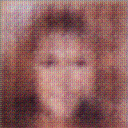
\includegraphics[width=150px]{500_fake_images/samples_5_247.png}%
\caption{A Man In A Suit And Tie Is Smiling}%
\end{figure}

%
\end{document}